\subsection{Kalibrierung der kleinen Scheibe}
Für die kleine Drehscheibe wurden alle $\unit[45]{^\circ}$ die resultierende Kraft bei einem Radius $r = \unit[(18.8 \pm 0.3)]{cm}$ gemessen (siehe Abbildung \ref{fig:kal1}). Mit linearer Regression\footnote{Berechnung durch Origin} bekommen wir eine Steigung von $d = \unit[(23.9 \pm 0.1)]{mN m}$.

Zudem kann die Winkelrichtgröße durch das hinzufügen von mehreren bekannten Trägheitsmomenten ($J_Z$) und im Anschluss mit Formel \ref{eq:wink} berechnet werden
\begin{equation}
T^2 = \frac{4\pi^2}{d}\cdot (J_0+J_Z)
\end{equation}

Durch Lineare Regression können wir die Steigung $W = \frac{4\pi^2}{d}$ ermitteln (siehe Abbildung \ref{fig:kal2}) und somit $d$ berechnen:
\begin{equation*}
d = \frac{4\pi^2}{W} = \unit[(22.3 \pm 0.3)]{mN cm}
\end{equation*}
Diese Werte weichen von der statischen Bestimmung leicht ab, Gründe hierfür können systematische Fehler der Kraftmessgeräte oder aber auch Reibung bei der Schwingung sein. Für die folgenden Berechnungen wurde der Wert durch die statische Bestimmung benutzt, da dieser weniger Fehlerquellen hat.

Der y-Achsenabschnitt $f = \unit[(0.57 \pm 0.06)]{s^2}$ ergibt sich durch die Regression, und somit ist $J_0$
\begin{align}
J_0 &= f^2\frac{d}{4\pi^2}\\
J_0 &= \unit[183.8 \pm 1.2]{g m^2}
\end{align}


\begin{figure}
\begin{center}
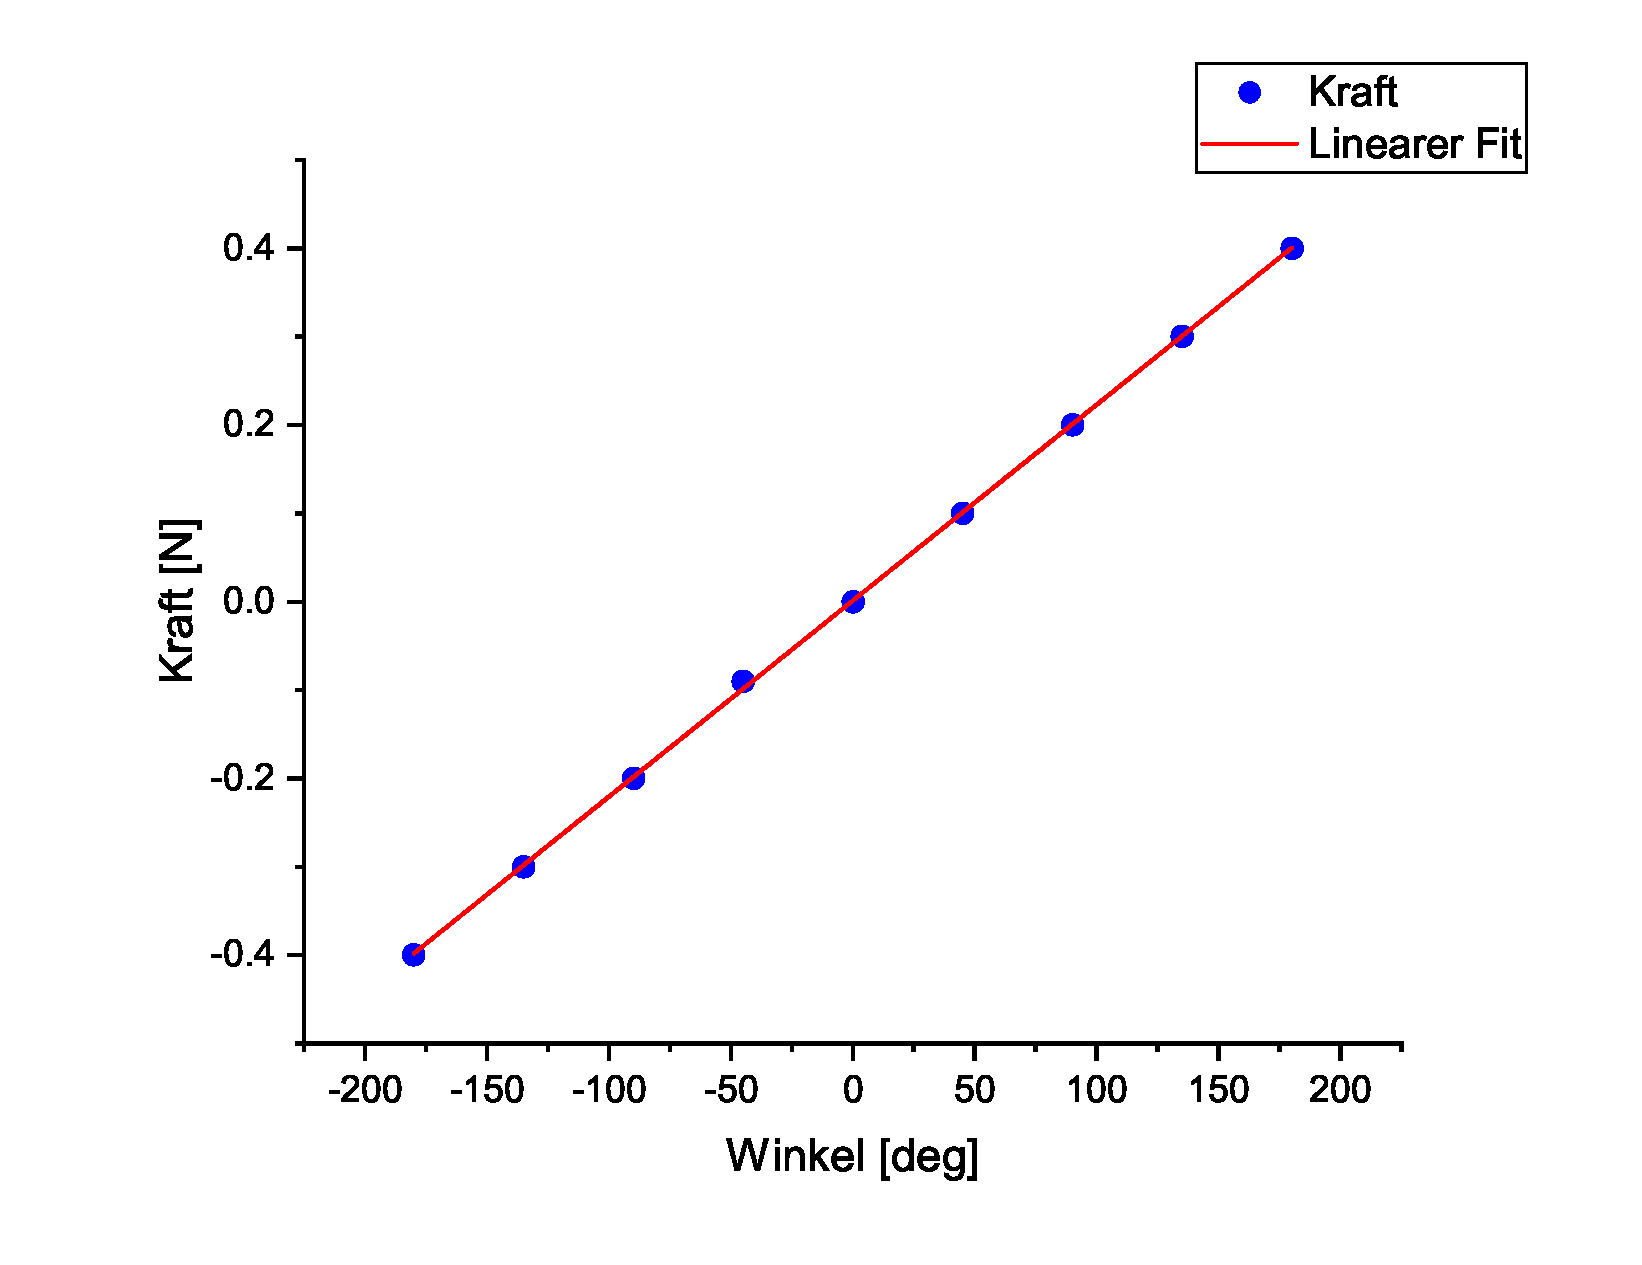
\includegraphics[width=0.7\textwidth]{Bilder/kal1.eps}
\caption{Statische Ermittlung der Winkelrichtgröße von der kleinen Scheibe}
\label{fig:kal1}
\end{center}
\end{figure}

\begin{figure}
\begin{center}
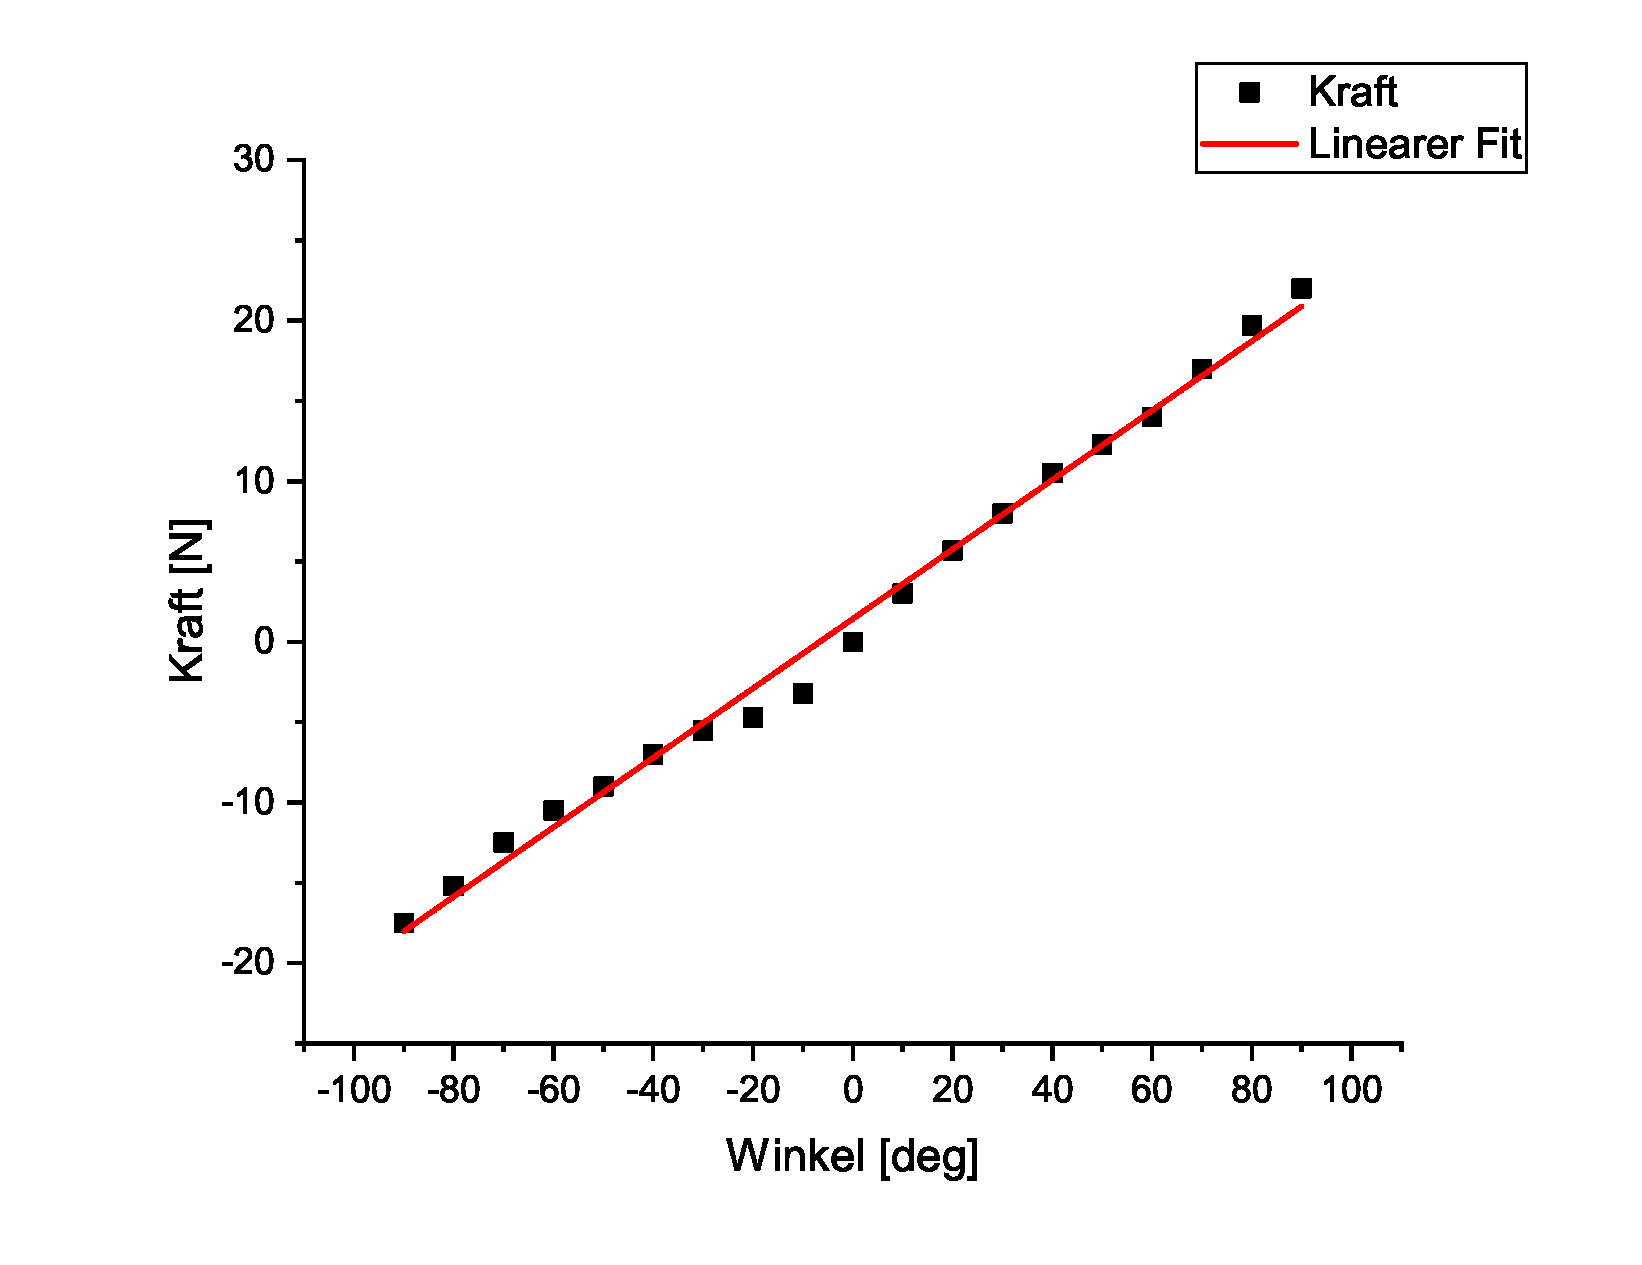
\includegraphics[width=0.7\textwidth]{Bilder/kal2.eps}
\caption{Dynamische Ermittlung der Winkelrichtgröße von der kleinen Scheibe}
\label{fig:kal2}
\end{center}
\end{figure}
